\documentclass[conference]{IEEEtran}
\usepackage{tikz}
\usepackage{pgfplots}
\usepackage{amsmath}
\usepackage{graphicx}
\usepackage{float}
\usepackage{subcaption}
\usetikzlibrary{shapes.geometric, arrows, positioning, fit, backgrounds}

\tikzstyle{startstop} = [rectangle, rounded corners, minimum width=3cm, minimum height=1cm, text centered, draw=black, fill=red!30]
\tikzstyle{process} = [rectangle, minimum width=3cm, minimum height=1cm, text centered, draw=black, fill=orange!30]
\tikzstyle{decision} = [diamond, minimum width=3cm, minimum height=1cm, text centered, draw=black, fill=green!30]
\tikzstyle{arrow} = [thick,->,>=stealth]
\tikzstyle{database} = [cylinder, shape border rotate=90, aspect=0.25, minimum width=2cm, minimum height=1.5cm, text centered, draw=black, fill=blue!30]
\tikzstyle{component} = [rectangle, minimum width=2.5cm, minimum height=1cm, text centered, draw=black, fill=yellow!30]

\begin{document}

\title{System Architecture and Workflow\\
Group Discussion Platform with Real-Time Video Conferencing}

\author{\IEEEauthorblockN{Research Paper Documentation}
\IEEEauthorblockA{System Design and Implementation}}

\maketitle

\section{System Architecture Overview}

\begin{figure}[H]
\centering
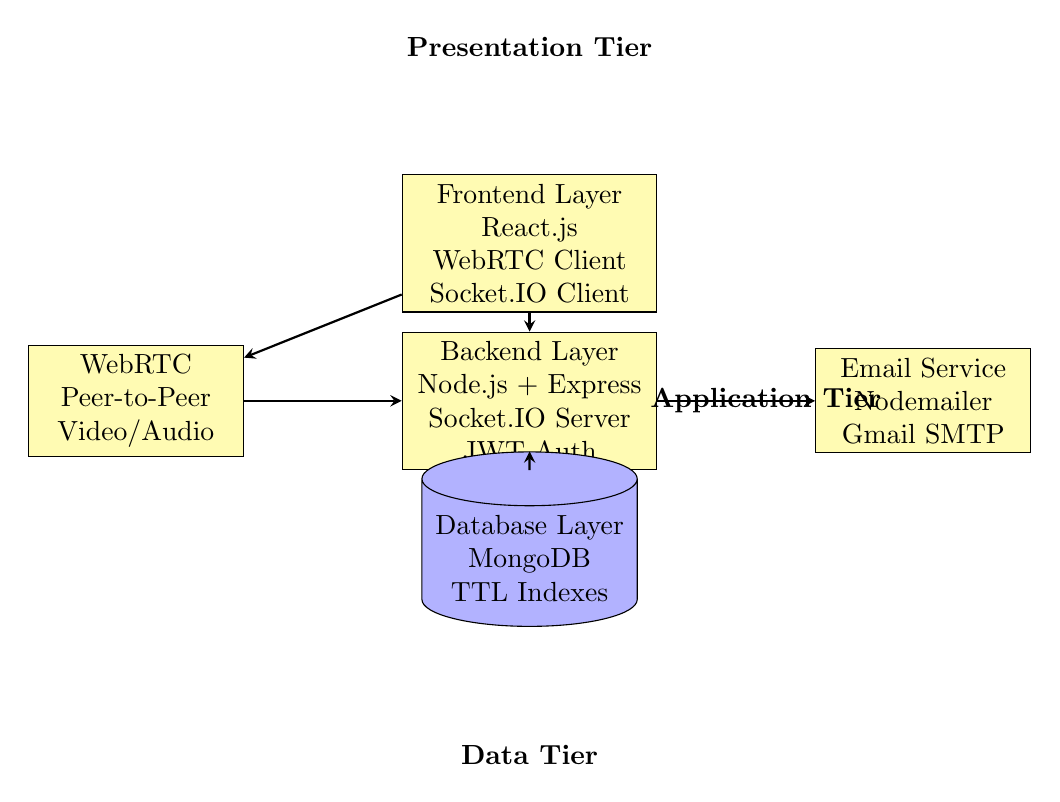
\begin{tikzpicture}[node distance=2cm]

% Frontend Layer
\node (frontend) [component, text width=3cm] {Frontend Layer\\React.js\\WebRTC Client\\Socket.IO Client};

% Backend Layer
\node (backend) [component, below of=frontend, text width=3cm] {Backend Layer\\Node.js + Express\\Socket.IO Server\\JWT Auth};

% Database Layer
\node (database) [database, below of=backend, text width=2.5cm] {Database Layer\\MongoDB\\TTL Indexes};

% External Services
\node (email) [component, right of=backend, xshift=3cm, text width=2.5cm] {Email Service\\Nodemailer\\Gmail SMTP};

% WebRTC Signaling
\node (webrtc) [component, left of=backend, xshift=-3cm, text width=2.5cm] {WebRTC\\Peer-to-Peer\\Video/Audio};

% Arrows
\draw [arrow] (frontend) -- (backend);
\draw [arrow] (backend) -- (database);
\draw [arrow] (backend) -- (email);
\draw [arrow] (frontend) -- (webrtc);
\draw [arrow] (webrtc) -- (backend);

% Layer Labels
\node [above of=frontend, yshift=0.5cm] {\textbf{Presentation Tier}};
\node [right of=backend, xshift=1cm] {\textbf{Application Tier}};
\node [below of=database, yshift=-0.5cm] {\textbf{Data Tier}};

\end{tikzpicture}
\caption{Three-Tier System Architecture}
\label{fig:architecture}
\end{figure}

\section{Component Architecture}

\begin{figure}[H]
\centering
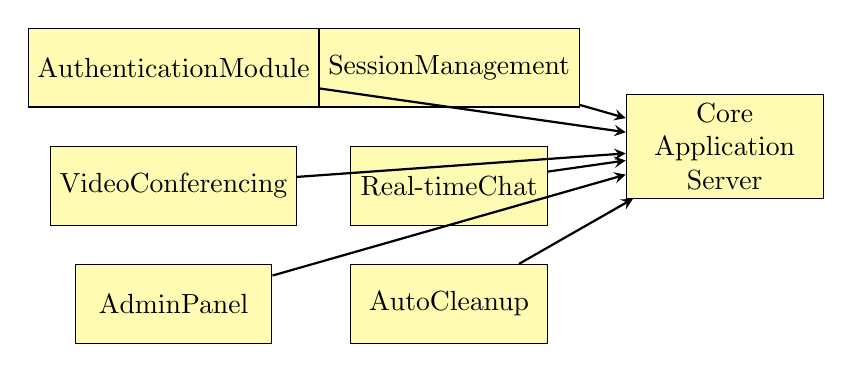
\begin{tikzpicture}[node distance=1.5cm]

% Main Components
\node (auth) [component] {Authentication\\Module};
\node (session) [component, right of=auth, xshift=2cm] {Session\\Management};
\node (video) [component, below of=auth] {Video\\Conferencing};
\node (chat) [component, right of=video, xshift=2cm] {Real-time\\Chat};
\node (admin) [component, below of=video] {Admin\\Panel};
\node (cleanup) [component, right of=admin, xshift=2cm] {Auto\\Cleanup};

% Central Hub
\node (core) [component, right of=session, xshift=2cm, yshift=-1cm, text width=2cm] {Core\\Application\\Server};

% Connections
\draw [arrow] (auth) -- (core);
\draw [arrow] (session) -- (core);
\draw [arrow] (video) -- (core);
\draw [arrow] (chat) -- (core);
\draw [arrow] (admin) -- (core);
\draw [arrow] (cleanup) -- (core);

\end{tikzpicture}
\caption{Component Architecture Diagram}
\label{fig:components}
\end{figure}

\section{User Authentication Workflow}

\begin{figure}[H]
\centering
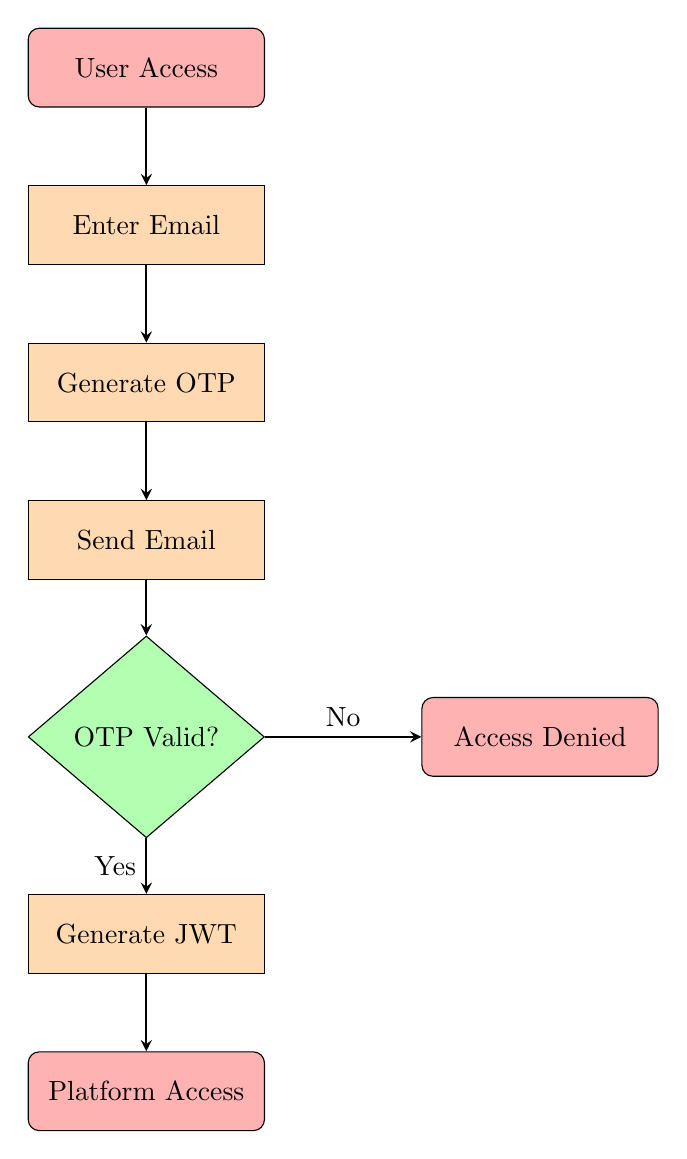
\begin{tikzpicture}[node distance=2cm]

\node (start) [startstop] {User Access};
\node (login) [process, below of=start] {Enter Email};
\node (otp_gen) [process, below of=login] {Generate OTP};
\node (send_email) [process, below of=otp_gen] {Send Email};
\node (verify) [decision, below of=send_email, yshift=-0.5cm] {OTP Valid?};
\node (jwt) [process, below of=verify, yshift=-0.5cm] {Generate JWT};
\node (access) [startstop, below of=jwt] {Platform Access};
\node (reject) [startstop, right of=verify, xshift=3cm] {Access Denied};

\draw [arrow] (start) -- (login);
\draw [arrow] (login) -- (otp_gen);
\draw [arrow] (otp_gen) -- (send_email);
\draw [arrow] (send_email) -- (verify);
\draw [arrow] (verify) -- node[anchor=east] {Yes} (jwt);
\draw [arrow] (verify) -- node[anchor=south] {No} (reject);
\draw [arrow] (jwt) -- (access);

\end{tikzpicture}
\caption{Authentication Workflow}
\label{fig:auth_workflow}
\end{figure}

\section{Session Management Workflow}

\begin{figure}[H]
\centering
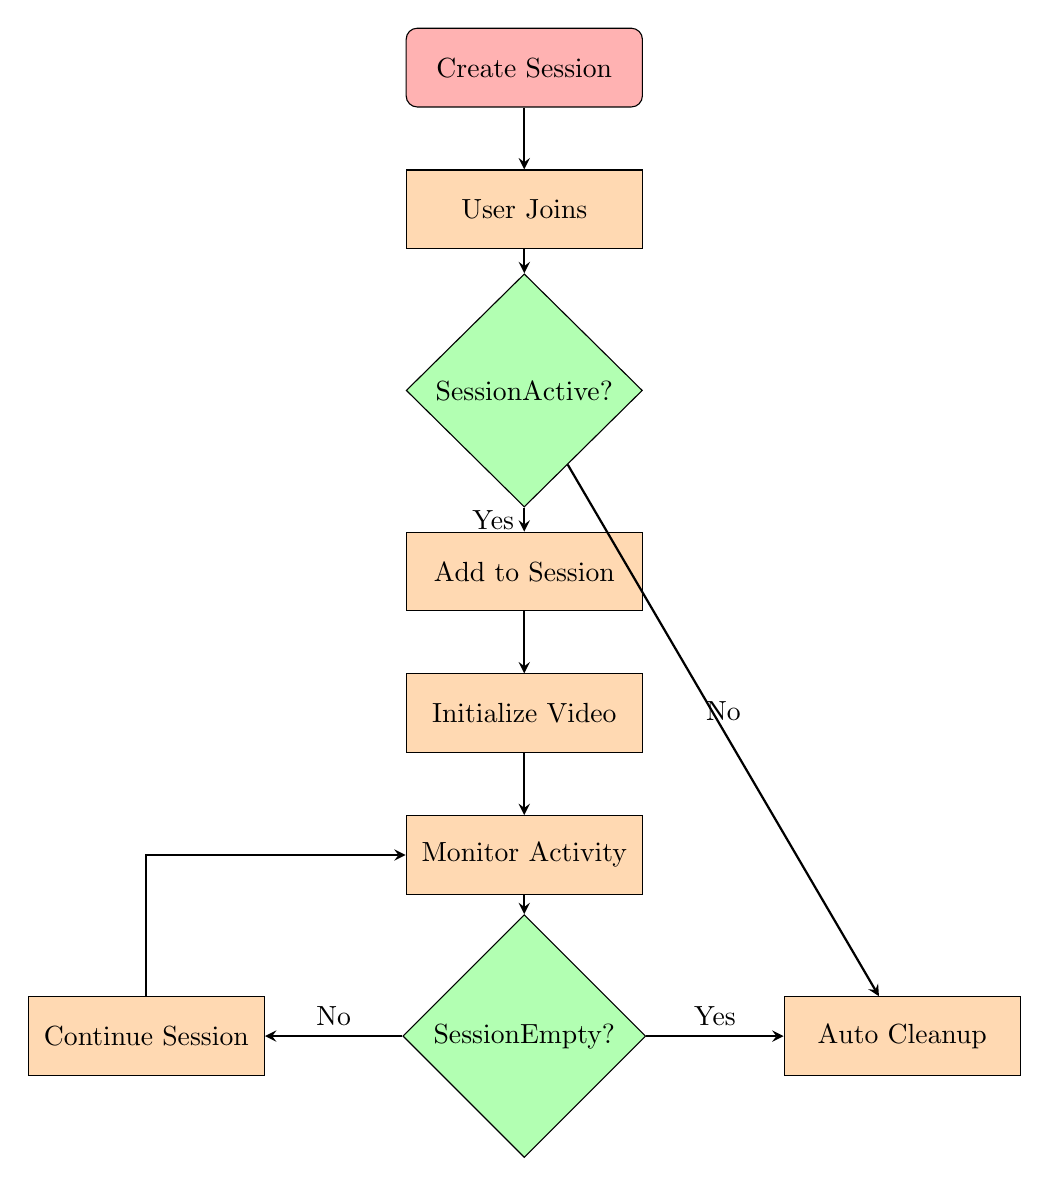
\begin{tikzpicture}[node distance=1.8cm]

\node (create) [startstop] {Create Session};
\node (join) [process, below of=create] {User Joins};
\node (check) [decision, below of=join, yshift=-0.5cm] {Session\\Active?};
\node (add_user) [process, below of=check, yshift=-0.5cm] {Add to Session};
\node (start_video) [process, below of=add_user] {Initialize Video};
\node (monitor) [process, below of=start_video] {Monitor Activity};
\node (cleanup_check) [decision, below of=monitor, yshift=-0.5cm] {Session\\Empty?};
\node (cleanup) [process, right of=cleanup_check, xshift=3cm] {Auto Cleanup};
\node (continue) [process, left of=cleanup_check, xshift=-3cm] {Continue Session};

\draw [arrow] (create) -- (join);
\draw [arrow] (join) -- (check);
\draw [arrow] (check) -- node[anchor=east] {Yes} (add_user);
\draw [arrow] (check) -- node[anchor=south] {No} (cleanup);
\draw [arrow] (add_user) -- (start_video);
\draw [arrow] (start_video) -- (monitor);
\draw [arrow] (monitor) -- (cleanup_check);
\draw [arrow] (cleanup_check) -- node[anchor=south] {Yes} (cleanup);
\draw [arrow] (cleanup_check) -- node[anchor=south] {No} (continue);
\draw [arrow] (continue) |- (monitor);

\end{tikzpicture}
\caption{Session Management Workflow}
\label{fig:session_workflow}
\end{figure}

\section{Real-Time Communication Flow}

\begin{figure}[H]
\centering
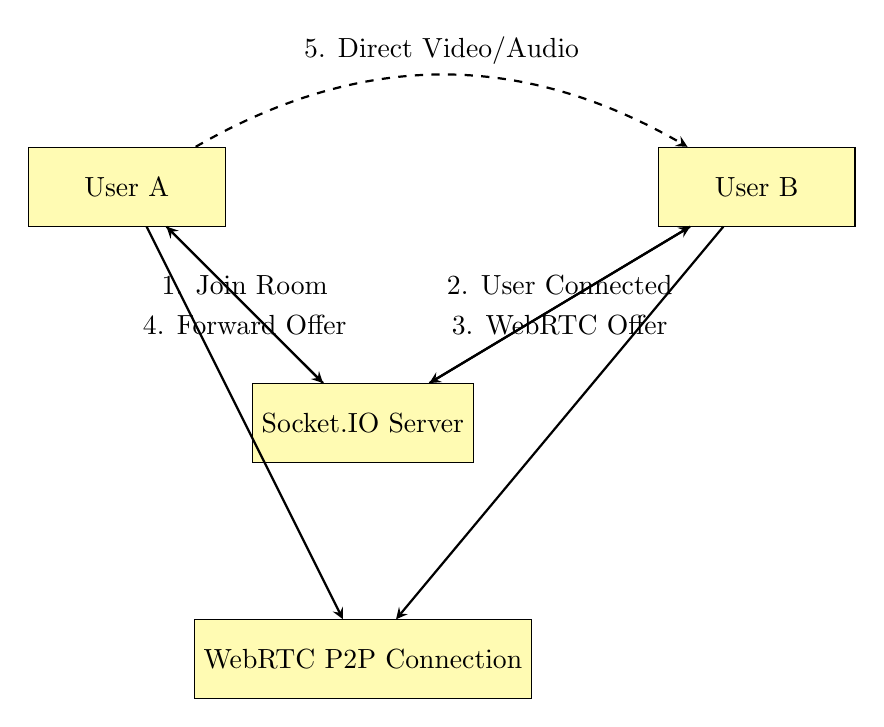
\begin{tikzpicture}[node distance=2cm]

% Users
\node (user1) [component] {User A};
\node (user2) [component, right of=user1, xshift=6cm] {User B};

% Server
\node (server) [component, below of=user1, xshift=3cm, yshift=-1cm] {Socket.IO Server};

% WebRTC
\node (webrtc_flow) [component, below of=server, yshift=-1cm] {WebRTC P2P Connection};

% Message Flow
\draw [arrow] (user1) -- node[above] {1. Join Room} (server);
\draw [arrow] (server) -- node[above] {2. User Connected} (user2);
\draw [arrow] (user2) -- node[below] {3. WebRTC Offer} (server);
\draw [arrow] (server) -- node[below] {4. Forward Offer} (user1);
\draw [arrow] (user1) -- (webrtc_flow);
\draw [arrow] (user2) -- (webrtc_flow);
\draw [arrow, dashed] (user1) to[bend left=30] node[above] {5. Direct Video/Audio} (user2);

\end{tikzpicture}
\caption{Real-Time Communication Flow}
\label{fig:communication_flow}
\end{figure}

\section{Database Schema Architecture}

\begin{figure}[H]
\centering
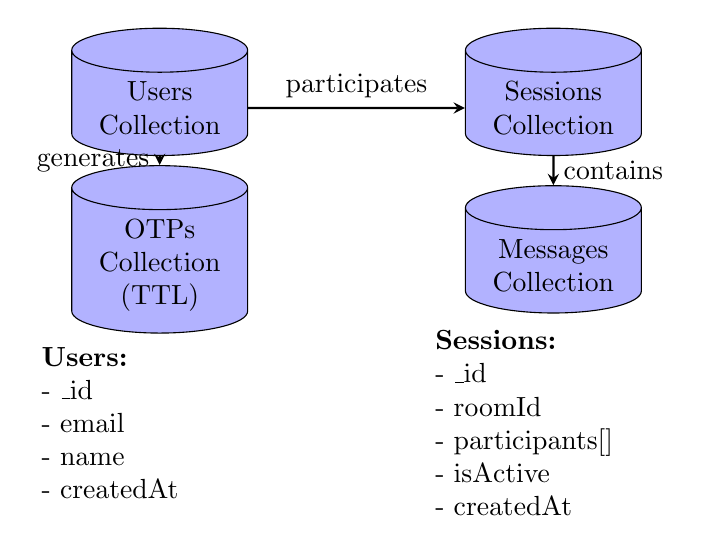
\begin{tikzpicture}[node distance=2cm]

% Collections
\node (users) [database, text width=2cm] {Users\\Collection};
\node (sessions) [database, right of=users, xshift=3cm, text width=2cm] {Sessions\\Collection};
\node (otps) [database, below of=users, text width=2cm] {OTPs\\Collection\\(TTL)};
\node (messages) [database, right of=otps, xshift=3cm, text width=2cm] {Messages\\Collection};

% Relationships
\draw [arrow] (users) -- node[above] {participates} (sessions);
\draw [arrow] (users) -- node[left] {generates} (otps);
\draw [arrow] (sessions) -- node[right] {contains} (messages);

% Schema Details
\node [below of=users, yshift=-2cm, text width=3cm, align=left] {
\textbf{Users:}\\
- \_id\\
- email\\
- name\\
- createdAt
};

\node [below of=sessions, yshift=-2cm, text width=3cm, align=left] {
\textbf{Sessions:}\\
- \_id\\
- roomId\\
- participants[]\\
- isActive\\
- createdAt
};

\end{tikzpicture}
\caption{Database Schema Architecture}
\label{fig:database_schema}
\end{figure}

\section{Deployment Architecture}

\begin{figure}[H]
\centering
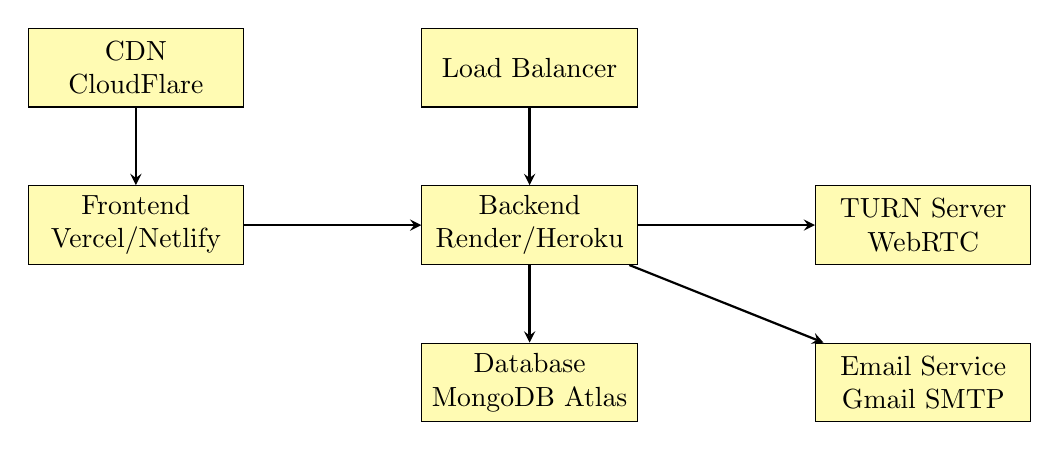
\begin{tikzpicture}[node distance=2cm]

% Cloud Services
\node (cdn) [component, text width=2.5cm] {CDN\\CloudFlare};
\node (frontend_host) [component, below of=cdn, text width=2.5cm] {Frontend\\Vercel/Netlify};
\node (backend_host) [component, right of=frontend_host, xshift=3cm, text width=2.5cm] {Backend\\Render/Heroku};
\node (db_host) [component, below of=backend_host, text width=2.5cm] {Database\\MongoDB Atlas};
\node (load_balancer) [component, above of=backend_host, text width=2.5cm] {Load Balancer};

% External Services
\node (turn_server) [component, right of=backend_host, xshift=3cm, text width=2.5cm] {TURN Server\\WebRTC};
\node (email_service) [component, below of=turn_server, text width=2.5cm] {Email Service\\Gmail SMTP};

% Connections
\draw [arrow] (cdn) -- (frontend_host);
\draw [arrow] (frontend_host) -- (backend_host);
\draw [arrow] (load_balancer) -- (backend_host);
\draw [arrow] (backend_host) -- (db_host);
\draw [arrow] (backend_host) -- (turn_server);
\draw [arrow] (backend_host) -- (email_service);

\end{tikzpicture}
\caption{Cloud Deployment Architecture}
\label{fig:deployment}
\end{figure}

\section{Performance Monitoring Workflow}

\begin{figure}[H]
\centering
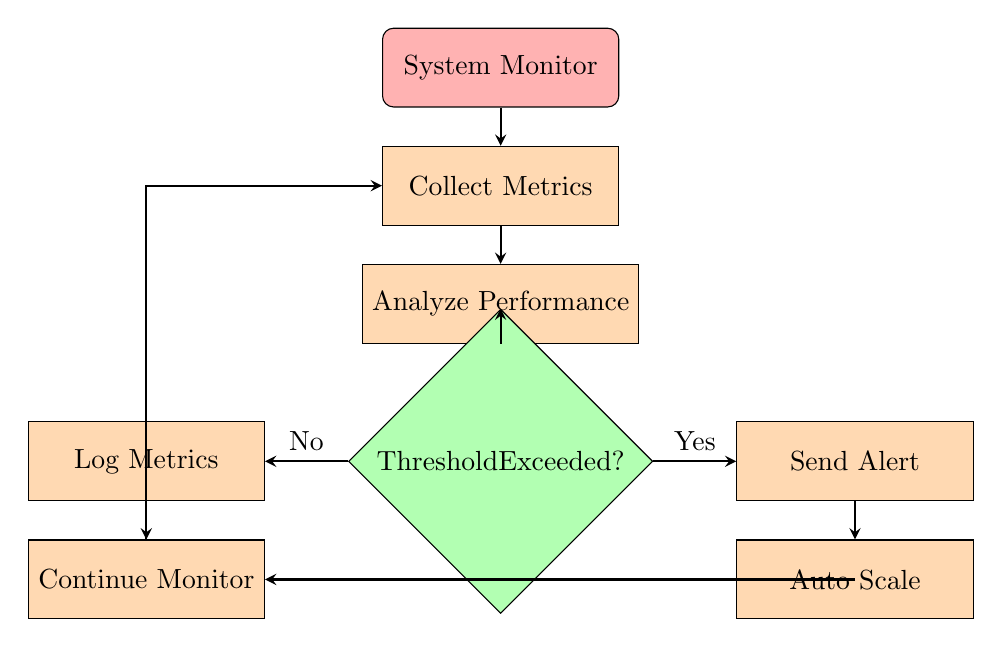
\begin{tikzpicture}[node distance=1.5cm]

\node (monitor) [startstop] {System Monitor};
\node (collect) [process, below of=monitor] {Collect Metrics};
\node (analyze) [process, below of=collect] {Analyze Performance};
\node (threshold) [decision, below of=analyze, yshift=-0.5cm] {Threshold\\Exceeded?};
\node (alert) [process, right of=threshold, xshift=3cm] {Send Alert};
\node (scale) [process, below of=alert] {Auto Scale};
\node (log) [process, left of=threshold, xshift=-3cm] {Log Metrics};
\node (continue) [process, below of=log] {Continue Monitor};

\draw [arrow] (monitor) -- (collect);
\draw [arrow] (collect) -- (analyze);
\draw [arrow] (analyze) -- (threshold);
\draw [arrow] (threshold) -- node[anchor=south] {Yes} (alert);
\draw [arrow] (threshold) -- node[anchor=south] {No} (log);
\draw [arrow] (alert) -- (scale);
\draw [arrow] (log) -- (continue);
\draw [arrow] (continue) |- (collect);
\draw [arrow] (scale) |- (continue);

\end{tikzpicture}
\caption{Performance Monitoring Workflow}
\label{fig:monitoring}
\end{figure}

\section{Security Architecture}

\begin{figure}[H]
\centering
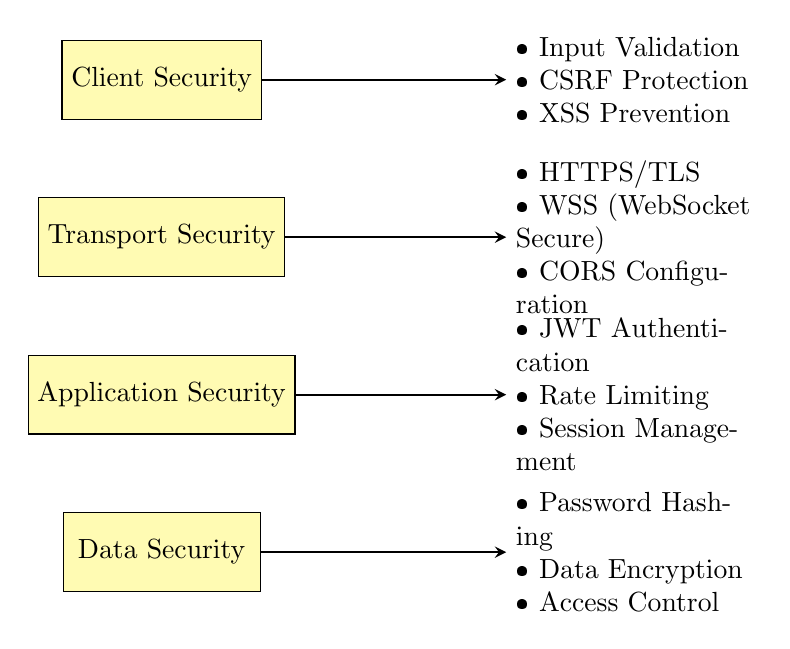
\begin{tikzpicture}[node distance=2cm]

% Security Layers
\node (client) [component] {Client Security};
\node (transport) [component, below of=client] {Transport Security};
\node (app) [component, below of=transport] {Application Security};
\node (data) [component, below of=app] {Data Security};

% Security Features
\node (client_features) [right of=client, xshift=4cm, text width=3cm, align=left] {
• Input Validation\\
• CSRF Protection\\
• XSS Prevention
};

\node (transport_features) [right of=transport, xshift=4cm, text width=3cm, align=left] {
• HTTPS/TLS\\
• WSS (WebSocket Secure)\\
• CORS Configuration
};

\node (app_features) [right of=app, xshift=4cm, text width=3cm, align=left] {
• JWT Authentication\\
• Rate Limiting\\
• Session Management
};

\node (data_features) [right of=data, xshift=4cm, text width=3cm, align=left] {
• Password Hashing\\
• Data Encryption\\
• Access Control
};

% Connections
\draw [arrow] (client) -- (client_features);
\draw [arrow] (transport) -- (transport_features);
\draw [arrow] (app) -- (app_features);
\draw [arrow] (data) -- (data_features);

\end{tikzpicture}
\caption{Multi-Layer Security Architecture}
\label{fig:security}
\end{figure}

\end{document}